\documentclass[border=8pt]{standalone}
\usepackage[utf8]{inputenc}
\usepackage{tikz}
\usetikzlibrary{shapes.geometric, positioning}

\tikzset{
  entita/.style     = {rectangle, draw, thick, fill=blue!8, minimum width=26mm, minimum height=9mm, font=\small},
  debole/.style     = {entita, double, double distance=1.5pt},
  relazione/.style  = {diamond, draw, thick, fill=orange!15, aspect=2, inner sep=1pt, font=\footnotesize},
  card/.style       = {font=\scriptsize, midway, fill=white, inner sep=1.5pt},
  link/.style       = {thick}
}

\begin{document}
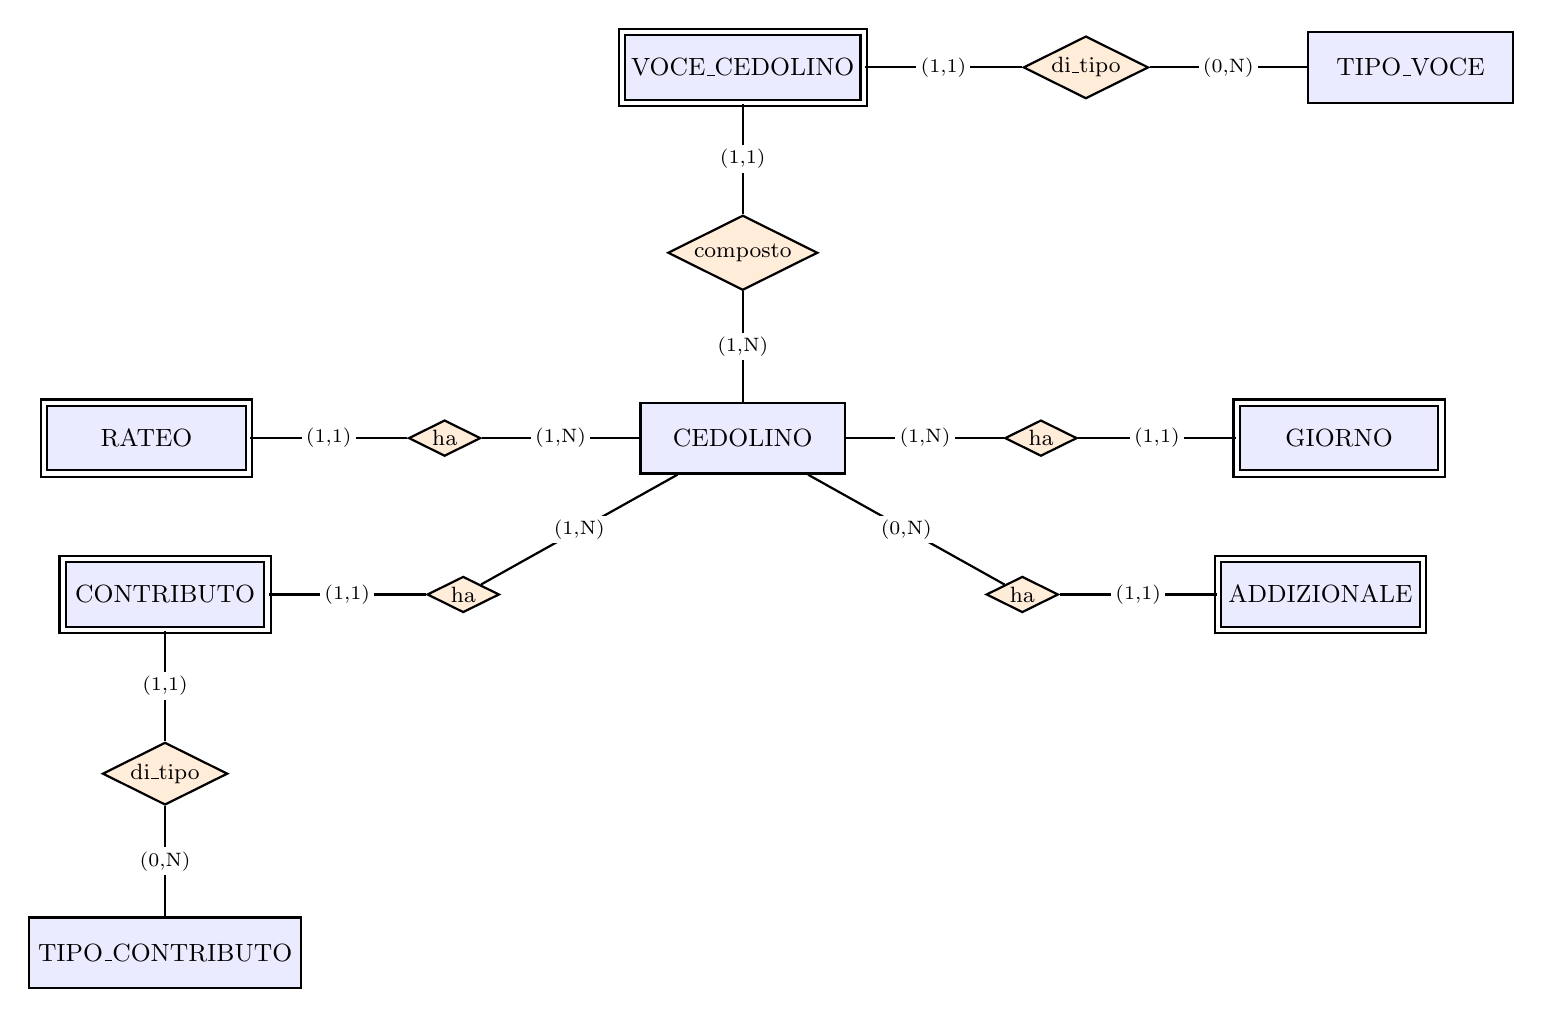
\begin{tikzpicture}[node distance=14mm and 20mm]

  \node[entita] (ced) {CEDOLINO};

  % voci + tipo voce (sopra)
  \node[relazione, above=of ced]      (comp)   {composto};
  \node[debole, above=of comp]        (voce)   {VOCE\_CEDOLINO};
  \node[relazione, right=of voce]     (dtv)    {di\_tipo};
  \node[entita, right=of dtv]         (tipov)  {TIPO\_VOCE};

  % ratei (sinistra)
  \node[relazione, left=of ced]       (harat)  {ha};
  \node[debole, left=of harat]        (rateo)  {RATEO};

  % giorni (destra)
  \node[relazione, right=of ced]      (hagio)  {ha};
  \node[debole, right=of hagio]       (giorno) {GIORNO};

  % contributi + tipo (basso sinistra)
  \node[relazione, below left=of ced] (hacon)  {ha};
  \node[debole, left=of hacon]        (contr)  {CONTRIBUTO};
  \node[relazione, below=of contr]    (dtc)    {di\_tipo};
  \node[entita, below=of dtc]         (tipoc)  {TIPO\_CONTRIBUTO};

  % addizionali (basso destra)
  \node[relazione, below right=of ced] (hadd)  {ha};
  \node[debole, right=of hadd]         (addz)  {ADDIZIONALE};

  \draw[link] (ced) -- (comp)  node[card]{(1,N)};
  \draw[link] (comp) -- (voce) node[card]{(1,1)};
  \draw[link] (voce) -- (dtv)  node[card]{(1,1)};
  \draw[link] (dtv) -- (tipov) node[card]{(0,N)};

  \draw[link] (ced) -- (harat)  node[card]{(1,N)};
  \draw[link] (harat) -- (rateo) node[card]{(1,1)};

  \draw[link] (ced) -- (hagio)  node[card]{(1,N)};
  \draw[link] (hagio) -- (giorno) node[card]{(1,1)};

  \draw[link] (ced) -- (hacon)  node[card]{(1,N)};
  \draw[link] (hacon) -- (contr) node[card]{(1,1)};
  \draw[link] (contr) -- (dtc)  node[card]{(1,1)};
  \draw[link] (dtc) -- (tipoc)  node[card]{(0,N)};

  \draw[link] (ced) -- (hadd)   node[card]{(0,N)};
  \draw[link] (hadd) -- (addz)  node[card]{(1,1)};

\end{tikzpicture}
\end{document}
